% !TEX TS-program = pdflatex
% !TEX encoding = UTF-8 Unicode

% This is a simple template for a LaTeX document using the "article" class.
% See "book", "report", "letter" for other types of document.

\documentclass[11pt]{article} % use larger type; default would be 10pt

\usepackage[utf8]{inputenc} % set input encoding (not needed with XeLaTeX)

%%% Examples of Article customizations
% These packages are optional, depending whether you want the features they provide.
% See the LaTeX Companion or other references for full information.

%%% PAGE DIMENSIONS
\usepackage{geometry} % to change the page dimensions
\geometry{a4paper} % or letterpaper (US) or a5paper or....
% \geometry{margin=2in} % for example, change the margins to 2 inches all round
% \geometry{landscape} % set up the page for landscape
%   read geometry.pdf for detailed page layout information

\usepackage{graphicx} % support the \includegraphics command and options

% \usepackage[parfill]{parskip} % Activate to begin paragraphs with an empty line rather than an indent

%%% PACKAGES
\usepackage{booktabs} % for much better looking tables
\usepackage{array} % for better arrays (eg matrices) in maths
\usepackage{paralist} % very flexible & customisable lists (eg. enumerate/itemize, etc.)
\usepackage{verbatim} % adds environment for commenting out blocks of text & for better verbatim
\usepackage{subfig} % make it possible to include more than one captioned figure/table in a single float
% These packages are all incorporated in the memoir class to one degree or another...

%%% HEADERS & FOOTERS
\usepackage{fancyhdr} % This should be set AFTER setting up the page geometry
\pagestyle{fancy} % options: empty , plain , fancy
\renewcommand{\headrulewidth}{0pt} % customise the layout...
\lhead{}\chead{}\rhead{}
\lfoot{}\cfoot{\thepage}\rfoot{}

%%% SECTION TITLE APPEARANCE
\usepackage{sectsty}


\allsectionsfont{\sffamily\mdseries\upshape} % (See the fntguide.pdf for font help)
% (This matches ConTeXt defaults)

%%% ToC (table of contents) APPEARANCE
\usepackage[nottoc,notlof,notlot]{tocbibind} % Put the bibliography in the ToC
\usepackage[titles,subfigure]{tocloft} % Alter the style of the Table of Contents
\renewcommand{\cftsecfont}{\rmfamily\mdseries\upshape}
\renewcommand{\cftsecpagefont}{\rmfamily\mdseries\upshape} % No bold!

%%% END Article customizations


\usepackage[bulgarian]{babel}
\usepackage{physics}
\usepackage{amsmath}
\usepackage{centernot}
\usepackage{enumitem}

%%% The "real" document content comes below...

\title{3.Крайни автомати. Регулярни езици. Теорема на Клини}
\author{Play4u}
%\date{} % Activate to display a given date or no date (if empty),
         % otherwise the current date is printed 

\begin{document}
\maketitle

\textbf{\textit{Конспект:}} Детерминирани крайни автомати. Регулярни операции. Недетерминирани крайни автомати. Представяне на всеки недетерминиран краен автомат с детерминиран такъв(с доказателство). Затвореност относно регулярните операции. Теорема на Клини(с доказателство). Лема за покачването (uvw) (с доказателство). Примери за регулярни и нерегулярни езици. Минимизация на състоянията. Теорема на Майхил-Нероуд(с доказателство). Алгоритъм за контруиране на минимален автомат, еквивалентен на даден детерминиран краен автомат.

\newcommand{\lrangle}[1]{\left\langle #1 \right\rangle}

\newcommand{\belongsTo}{\in}
\newcommand{\notBelongsTo}{\centernot\in}
\newcommand{\kda}{A = <Q, X, q_{0}, \delta, F>}

\newcommand{\italicBold}[1]{\textbf{\emph{#1}}}
\newcommand{\definition}{\italicBold{Дефиниция:}}
\newcommand{\theorem}{\italicBold{Теорема:}}
\newcommand{\lemma}{\italicBold{Лема:}}
\newcommand{\proof}{\italicBold{Доказателство:}}

\newcommand{\curlies}[1]{\{#1\}}

\section{Формални езици(опционално)}

Нека $X = \{x_1, x_2, ..., x_n\}$ е крайна азбука, $X^*$ е множеството от всички думи над $X$, $X_{*}$ е множеството от всички думи над $X$, а $X^{+} = X^{k}$ 
- множеството от думите с дължина 
$k$, $X^{1} = X$, а $X^{0}$ 
се състои само от $\varepsilon$. \par

Всяко от множествата $X^{k}, k = 0, 1, 2 ...$ е крайно $\abs{X^{k}} = \abs{X}^{k}$ и тъй като $X^{*} = X^{0} \cup X^{1} \cup X^{2}...$ е обединение на изброима фамилия изброими множества можем да приложим Теорема 1.3.1 (need citation) и да получим следното \par

\textbf{Следствие 4.1.1}: \emph{Множеството $X^{*}$ от думите над крайната азбука $X$ е изброимо} \par
   

\section{Крайни детерминирани автомати}
Формалните езици по естествен начин дефинират езици над множеството си терминални символи. Те обаче не позволяват да се даде по един достатъчен ясен начин отговор на въпроси от вида "Даден e език чрез граматиката си $\Gamma = \left\langle N, T, S, P \right\rangle$"
и дума $\alpha \epsilon \Gamma^*.$ Принадлежи ли $\alpha$ на $\Gamma?$" \par

\subsection{Регулярни операции}
За целта можем да използваме т.нар. абстрактни математически машини. Всяка една такава машина можем да разглеждаме като черна кутия, която чете от входа дума над дадена азбука и може да изведе на изхода дума над друга (не непременно различна от входната азбука). Характерно е, че във всеки момент от работата си машината се намира в някакво състояние q, принадлежащо ня крайно множество $Q$ от състояния. Смяната на едно състояние в друго става в изброимо множество от моменти на времето, наричани тактове. Между всеки два такта машината остава в едно и също състояние. Новото състояние се определя еднозначно от текущото състояние и входната буква, която машината чете в този момент. Изходната буква, когато машината действително извежда нещо, също е функция на текущото състояние и входна буква. \par

В началото машината винаги се намира в едно и също състояние, наричано "начално състояние". Работата й се определя от цикличното повтаряне на няколко прости действия - прочитане на входна буква, определяне на от тази буква и текущото състояние на изходна буква и следващото състояние, извеждане на изходната буква и смяна на текущото състояние със следващото, изчакване до настъпване на следващият акт, когато действията се повтарят отново. \par

Абстрактната машина може да завърши работа, кгоато достигне някое от предварително фиксираните заключителни състояния или когато функцията, определяща следващото състояние е частична (машината не може да продължи да работи заради недефинираност). Разбира се, спирането може да се извърши и при проичтането на входна дума докрай или при някое друго, свързано с конкретната дефиниция събитие. Има машини, които са в състояние никога да не завършат работа при определени обстоятелства. \par 

\textbf{\emph{Дефиниция:}} \emph{Краен детерминиран автомат (КДА) наричаме петорката} \\
\centerline{$A = \lrangle{Q, X, q_{0}, \delta, F}$}\\
в която: $Q$ е крайно множество от състояния; $X$ е крайна входна азбука; $q_{0} \epsilon Q$ е начално състояние; 
$\delta : Q \times X \to Q$ е частична функция на прходите, пресмятаща следващото състояние; $F \subseteq Q$ са заключителните състояния на КДА. \par

Можем да представим КДА чрез краен ориентиран мултиграф, с върхове елементите на Q, в който върхът $q_{i} \epsilon Q$ и върхът $q_{j} \epsilon Q$ са свързани с ребро, надписано с $x \epsilon X$, ако $\delta(q_{i}, x) = q_{j}$.

\italicBold{Дефиниция:} Казваме, че КДА 
$\kda $ с разширена функция на преходите 
$\Delta$ разпознава думата 
$\alpha \belongsTo X^{*}$, ако $\Delta(q_{0}, \alpha) \belongsTo F$. Множеството 
$L_{A} = \{\alpha| \alpha \belongsTo X^{*}, \Delta(q_{0}, \alpha) \belongsTo F\}$ наричнаме език, разпознаван от крайния детерминиран автомат $A$ \par

Ако функцията $\delta$ на КДА $\kda$ не е тотална, тогава можем да разширим $A$ до автомата 
$A' = < Q' = Q \cup \{q^{*}\}, X, q_{0}, \delta', F>$, такъв че 
$q^{*} \centernot\in F, \delta' : Q' \times X \to Q'$, а
$\delta'(q, x) = 
	\begin{cases}
		\delta(q,x) \quad \text{ако } \delta(q,x) 
		\text{ е дефинирана}\\
		q^{*} \quad \quad \quad \text{ако } \delta(q,x)
		\text{ не е дефинирана} \\
	\end{cases}$\par
Всички думи, разнознавани от $А$ се разпознават и от $A'$. Всяка дума $\alpha$, за която 
$\Delta_{A}(q_{0},\alpha) \notBelongsTo F$, и значи не се разпознава от $A$ - не се разпонзава и от $A'$, а за всяка дума $\beta$, за която 
$\Delta_{A}(q_{0}, \beta) не е дефинирана$ в $A'$ имаме
$\Delta_{A'}(q_{0}, \beta) = q^{*} \notBelongsTo F$ и $\beta$ отново не се разпознава. \\
Така $L_{A} = L_{A'}$ и следователно можем да работим и с недодефинирани автомати или да ги додефинираме (без да изменяме езика им), когато това е необходимо. \par
Сега ще покажем каква е връзката между КДА и автоматните езици\\
\italicBold{Теорема:} За всеки КДА, $\kda$ съществува авоматна граматика $\Gamma$ такава, че $L_{\Gamma} = L_{A}$\\

\section{Крайни недетерминирани автомати}
\italicBold{Дефиниция:} Петорката $\kda$, където $Q, X, q_{0}$ и $F$ са дефинирани както при КДА, а функцията на преходите е $\delta : Q \times X \to 2^{Q}$, наричаме краен недетерминиран автомат (КНА) \par

КНА работи по следния начин: Когато в резултат на изчисление на фунцкията $\delta$ се получи множеството $Q'$ от състояния в които КНА трябва да премине, той се размножава в $|Q'|$ копия и всяко копие преминава в едно от състоянията на $Q'$. \textbf{Можем да си мислим, че автоматът едновременно се намира във всичките състония на $Q'$.} Когато КНА прочете следващата буква, всяко от копията се разможава в толкова нови копия, колкото текущото му състояние, входната буква и функцията $\delta$ определят и всяко едно копие преминава в съответното състояние. Множеството от състояния в които се намира КНА ще съдържа състоянията на всички получени копия. Тази дефиниция ще уточним формално по следния начин. \par


\italicBold{Дефиниция:} Казваме, че КНА $A$ разпознава думата $\alpha \belongsTo X^{*}$, ако $\Delta(q_{0}, \alpha) \cap F \neq \emptyset$. Език, разпознаван от КНА $А$ определяме като \\
\centerline{$L_{A} = \{\alpha|\alpha \belongsTo X^{*}, \Delta(q_{0}, \alpha)\cap F \neq \emptyset \}$}

\theorem \emph{За всяка автоматна граматика $\Gamma$ съществува КНА $A$, такъв че $L_{\Gamma} = L_{A}$.}\\
\centerline{\emph{Insert proof here:}}

\theorem \emph{За всеки КНА $A$ съществува КДА $A'$ такъв, че $L_{A} = L_{A'}$}

\proof Нека $\kda$. Построяваме КДА 
$A' = < Q', X, t_{0}, \delta', F'$, където $Q' \subseteq 2^{Q}$. Нека множеството 
$\{q_{p1}, q_{p2}, ..., q_{pl} \} \belongsTo Q'$. За по кратко ще го означаваме с 
$t_{[p1, p2,..., pl ]}$. При това изначение определяме 
$t_{0} = \{q_{0}\} = t_{|0|}.$. Нека 
$F' = \{t_{[p1, p2, ..., pl]}|\{ q_{p1}, q_{p2}, ..., q_{pl} \}
\cap F \neq \emptyset\}, a \delta'(t_{[p1, p2, ... ,pl]}, x) = 
t_{[r1, r2, ..., rm]}, \text{ ако } \{q_{r1}, q_{r2}, ..., q_{rm}\}
= \cup_{i = 1}^{l}\delta(q_{pi}, x)$. Забележете, че не можем да фиксираме в явен вид кои точно подмножества на $Q$ влизат в $Q'$. Те се определят от изчисляването на функцията $\delta'$, започвайки от $\delta'(t_{|0|}, \alpha), \forall x \in X$. 
С индукция по дължината на $\alpha$ ще покажем, че $\Delta_{A'}(t_{|0|}, \alpha) = t_{[p1, p2, ..., pl]} \Leftrightarrow 
\Delta_{A}(q_{0}, \alpha) = \{q_{p1}, q_{p2}, ..., q_{pl}\}$.

\renewcommand{\theenumi}{\alph{enumi}}
\begin{enumerate}
	\item Нека $\omega = \epsilon$. Тогава $\Delta_{A'}(t_{|0|}, \epsilon) = t_{|0|}, a \Delta_{A}(q_{0}, \epsilon)= \{q_{0}\}$ и твърдението е в сила
	\item Допускаме верността на твърдението за някоя дума $\alpha$  и ще покажем, че $\Delta_{A'}(t_{t|0|}, \alpha x) = t_{[r1, r2, ..., rm]} \leftrightarrow \Delta_{A}(q_{0}, \alpha x) = 			\{q_{r1}, q_{r2}, ..., q_{rm}\}$.
	\item Нека $\Delta_{A'}(t_{|0|}, \alpha x) = t_{[r1, r2, ..., rm]}$, като
		$\Delta_{A'}(t_{|0|}, \alpha) = t_{[p1, p2, ..., pl]}$. Тогава $\delta'(t_{[p1, p2, ..., pl]}, x) = t_{[r1, r2, ...,rm]}$ и съгласно построението на $\delta'\{q_{r1}, q_{r2}, 				..., q_{rm} \} = $
		$\cup_{i=1}^{l}\delta(q_{pi}, x).$ Но от индуктивното допускане 
		$\Delta_{A}(q_{0}, \alpha) = \{q_{p1}, q_{p2}, ..., q_{pl}\} $ и следователно 
		$\Delta_{A}(q_{0}, \alpha x) = \{q_{r1}, q_{r2}, ..., q_{rm} \}$. Разсъжденията в другата посока са подобни.
\end{enumerate} \par

Като вземем предвид дефиницията на $F'$ и току що доказаното, получаваме $\Delta_{A'}(t_{|0|}, \alpha) \in F' \leftrightarrow 
\Delta_{A}(q_{0}, \alpha) \cap F \neq \emptyset$ и значи 
$L_{A'} = L_{A}$   

\section{Затвореност относно регулярните операции}
\begin{itemize}[noitemsep]
	\item Сечение: Ако $L_{1}$ и $L_{2}$ са два произволни автоматни езика над азбуката $\Sigma$, то $L_{1}\cap L_{2}$ също е автоматен език.
	\item Допълнение: Ако $L$ е автоматен език, то $\Sigma^{*}\setminus L$ също е автоматен.
	\item Обединение: Ако $L_{1}$ и $L_{2}$ са два произволни автоматни езика, то $L_{1}\cup L_{2}$ също е автоматен език.
\end{itemize}

\section{Регулярни езици}
\subsection{Примери за регулярни езици}
$a^{*}b^{*}$ - регулярен език\\
$\curlies{w \in \curlies{a,b}^{*}}$: всяко $a$ да е веднага последвано от $b$ е регулярен език.\\\\
Регулярни изрази(опционално):\\
$ \begin{array}{ll}%
	\text{Израз}  &  \text{Език}  \\
	a & \curlies{a} \\
	a + b & \curlies{a,b} \\
	a(a + b) & \curlies{aa, ab} \\
	a^{*} & \curlies{\epsilon, a, a^{2}, ..., a^{i}, ...} \\
	a^{*}(a + b) & \curlies{a, b, aa, ab, a^{2}a, a^{2}b, ..., a^{i} a, a^{i}b, ...} \\
	(a + b)^{*} & X^{*} \\                                           
	a^{*}b + b^{*}a & \curlies{b, a, ab, ba, a^{2}b, b^{2}a, ..., 	 a^{i}b, b^{i}a, ...}
\end{array}$%

\subsection{Примери за нерегулярни езици}
$a^{n} b^{n}: n \geq 0$\\
$\curlies{w \in \curlies{a,b}^{*}}$: всяко $a$ да има съотвестващо $b$ някъде в стринга, не е.

\subsection{Теорема на Клини} 
\emph{Множествата на регулярните и автоматните езици съвпадат}

\proof 
\renewcommand{\theenumi}{\arabic{enumi}}
\begin{enumerate}
	\item Ще покажем s индукция по дефиницията на регулярни езици, че всеки регулярен език е автоматен. Действително $\curlies{\epsilon, \emptyset} \text{ и } \curlies{x_{i}, i 				= 1,2,...,n}$ са автомарни езици, защото са крайни. Ако 				допуснем, че регулярните езици $L_{\alpha}$ и $L_{\beta}$, 				съответни на регулярните изрази $\alpha$ и $\beta$ са 					автоматни тогава
		$L_{\alpha} + L_{\beta}, L_{\alpha}.L_{\beta}$ и $L_{\alpha} ^{*}$ са автоматни, защото са сума, произведение и итерация на автоматни езици, съответно. Тъй като други регулярни 				езици няма, всеки регулярен език е автоматичен. 
	\item Нека езикът $L$ е автоматен. Ще докажен, че $L$ е регулярен език. Съществува КДА $\kda$ такъв, че $L = L_{A}$. Нека автоматът $A$ e представен с крайния ориентиран 					мултиграф $G$. Нека състоянията на $А$ са $Q = 							\curlies{q_{0}, q_{1}, ..., q_{n}}$ и $F = \curlies{q_{p1}, 			q_{p2}, ..., q_{pr}}$. 
		Да означим с $R_{ij}^{k}$ множеството от маршрутите в $G$ от връх $q_{i}$ до връх $q_{j}$, които не използват като вътрешни върхове $q_{k}, q_{k+1}, ..., q_{n}$.
		Очевидно, всеки маршрут от $q_{i}$ до $q_{j}$ означава определена дума $\alpha \in X^{*}$, такава че $\Delta(q_{i}, \alpha) = q_{j}$. Tака на множеството от маршрути $R_{ij}				^{k}$ можем да гледаме като на множество от съответните думи 		от $X^{*}$, т.е. $R_{ij}^{k}$ e език над $X^{*}$ - маршрутен 		език. В автомата няма състояния с номера по-големи от $n$ и 			затова $R_{ij}^{k}$ е езикът на всички маршрути от $q_{i}$ 				до $q_{j}$, когато $k > n$.
\end{enumerate}
		
\subsection{Минимизация на КДА}
\definition Крайните детерминирани автомати $A$ и $A'$ наричаме еквивалентни, ако $L_{A} = L_{A'}$ \par

Естествено е желанието, когато език се разпознава от повече от един автомат, да се опитаме да намерим този разпознавател, който е най-прост.\\
\definition КДА $A_{0}$, разпознаващ автоматния език $L$, наричаме \emph{минимален} за езика $L$, ако за всеки друг автомат $A$, разпознаващ $L$, $|Q_{0}| \leq |Q|$, където $Q$ и $Q_{0}$ са множествата от състояния на $A_{0}$ и $A$ съответно. \par

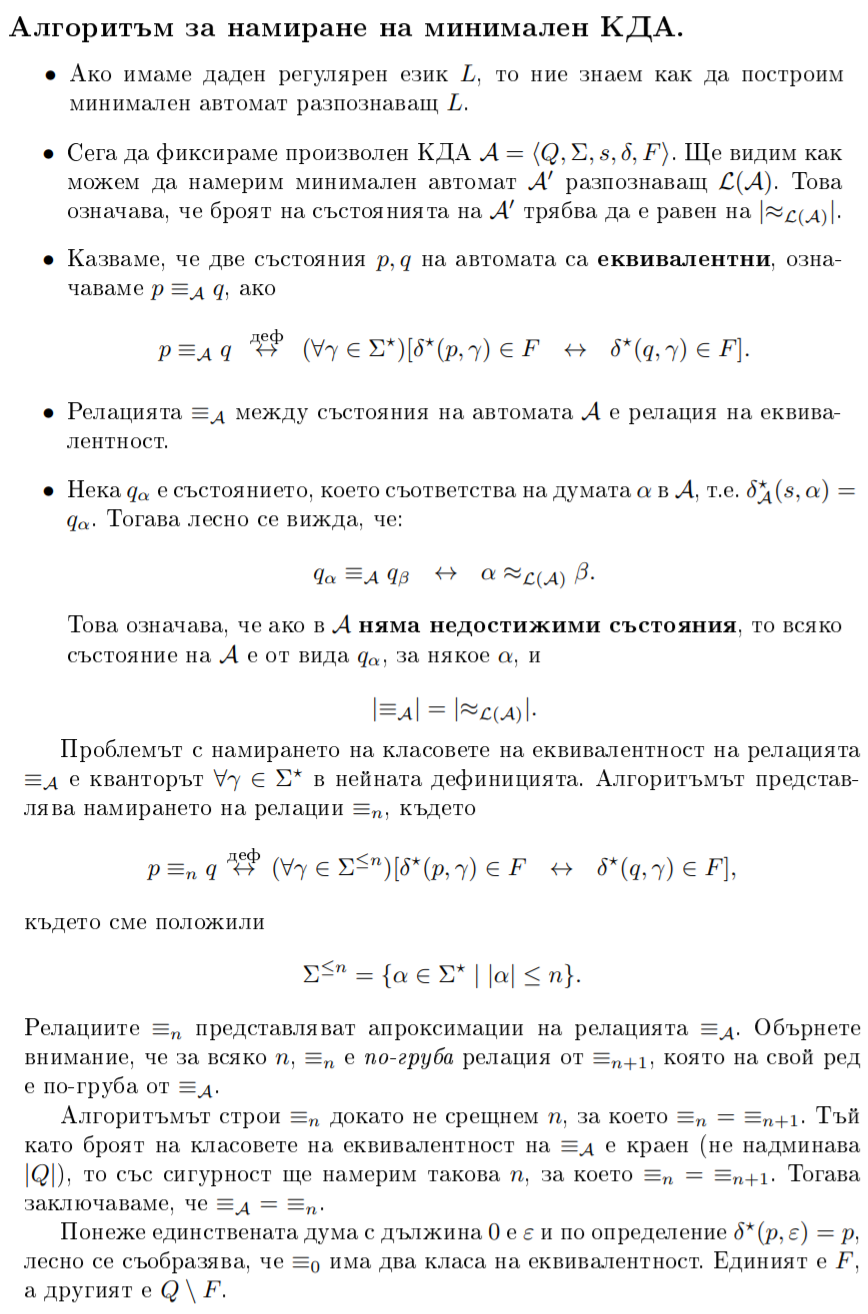
\includegraphics[scale=0.8]{MinKDAAlg.png}

\subsection{Теорема на Майхил-Нерод}
\emph{Нека $L \subseteq X^{*}$. Релацията $R_{L} \subseteq X^{*} \times X^{*}$ има краен индекс $\leftrightarrow e автоматен$}.

\proof
\renewcommand{\theenumi}{\arabic{enumi}}
\begin{enumerate}
	\item Нека $L$ е автоматен език. Тогава съществува КДА $\kda$, който разпознава $L$. Без ограничение на общността можем да счиаме, че сме освободили от ндеостижимите състояния на $A$, което не се отразява на неразпознаваемия език. Образуваме релацията $R_{A}$. Нека $(\alpha, \beta) \in R_{A}$. Ще покажем, че $(\alpha, \beta) \in R_{L}$. От $(\alpha, \beta) \in R_{A}$ следва $\Delta(q_{0}, \alpha) = \Delta(q_{0}, \beta).$ Нека $\gamma \in X^{*}$. Тогава $\Delta(q_{0}, \alpha \gamma) = \Delta(\Delta(q_{0}, \alpha), \gamma)
	= \Delta(\Delta(q_{0}, \beta), \gamma) = = \Delta(q_{0}, \beta \gamma = q.)$
	Или $q \in F$ и тогава $\alpha \gamma \in L$ и $\beta \gamma \in L$, или $q \notin F$ и тогава $\alpha \gamma \notin L$ и $\beta \gamma \notin L$.
	Следователно $(\alpha, \gamma) \in R_{L}$. От тук получаваме, че всеки клас на еквивалентност на $R_{A}$ се съдържа в клас на еквивалентност на $R_{L}$ или $IX(R_{L}) \leq IX(R_{A}) = |Q_{A}|$. Следователно $IX(R_{L})$ е краен
	\item Нека $IX(R_{L})$ е краен и $IX(R_{L}) = m$. Да означим с $[\alpha]$ класа на еквивалентност на $R_{L}$, съдържащ думата $\alpha \in X^{*}$. 
	Да означим с $Q = \curlies{[\epsilon], [\alpha_{1}, ... , [\alpha_{m-1}]}$ множеството от класовете на еквивалентността $R_{L}$, където $\alpha_{0} = \epsilon, \alpha_{1}, ..., \alpha_{m-1}$ са представители на съответните класове.
	 Образуваме КДА $A = < Q, X, [\epsilon], \delta, F >$, където $F = \curlies{[a_{p1}], [a_{p2},...,[a_{pr}]}$ са всички класове на еквивалентност на $R_{L}$, съдържащи само думи от езика на $L$. Ясно е от дефиницията на $R_{L}$, че всички думи от един и същ клас на $R_{L}$ едновременно са или не са в $L$, така че дефиницията на $F$ е коректна. 
	 Функцията на преходите $\delta$ дефинираме по следния начин: $\delta([\alpha], x) = [\alpha x]$. Тази дефиниция също е коректна, защото $\forall \beta \in [\alpha], [\beta x] = [\alpha x]$, заради дясната инвариантност на $R_{L}$.
	 \\ \\
	 {Докажи, чрез индукция по дължината на $\beta \in X^{*}$, че за разширената функция на преходите $\Delta$ на $A$ е в сила $\Delta([\alpha], \beta) = [\alpha \beta]$}.
	 \\ \\ 
\end{enumerate} \par

Ще докажем, че КДА $A$ разпознава точно езика $L$\\
\renewcommand{\theenumi}{\alph{enumi}}

\begin{enumerate}
	\item Нека $\omega \in L_{A}$, т.е. $\Delta([\epsilon], \omega) \in F. \text{ Но } \Delta([\epsilon], \omega) = [\epsilon \omega] = [\omega]$, т.е съществува $p_{j}, [\omega] = 					[\alpha_{pj}]$. Но тогава$\omega \in L$, защото всички думи 			на $[\alpha_{pj}]$ са от $L$ според дефиницията на $					[\alpha_{pj}]$.\\
	\item Нека $\omega \in L$. Тогава $[\omega] = [\alpha_{pj}]$ за някое $p_{j}$ и $\Delta([\epsilon], \omega) = [\omega] = [\alpha_{pj}]\in F$. Следователно $\omega \in L_{A}$. \\
\end{enumerate}\par

	Следователно езикът $L$ е автоматен \par
	Така построеният автомат е минимален КДА, разпознаващ $L$ както и нещо повече, което ще обясним по-надолу.\\
	\definition КДА $\kda$ и $A' = < Q', X, q_{0}', \delta', F'>$ са \emph{изоморфни}, ако съществува биекция $f : Q \to Q'$, такава че $f(q_{0}) = q_{0}'$ и $\forall \alpha \in X$ е в сила $\Delta(q_{0}, \alpha) = q' \leftrightarrow \Delta'(q_{0}', \alpha) = f(q')$. \\
	\theorem Автоматът $\kda$, построен в Теоремата на Майхил-Нерод е минимален за езика $L$ и всеки друг автомат за $L$ със същия брой състояния е изоморфен на $A$\\
	\centerline{\emph{Insert proof here}}

\section{uvw - теорема}
Спомага за показването на ограничеността на автоматните езици  и позволява да откриваме езици които не са автоматни\\
\theorem \emph{\textbf{(uvw-Теорема)}За всеки непразен автоматен език $L$ съществува цяло положеително число n такова, че ако $\alpha \in L$ и $d(\alpha) > n$, то $\alpha = uvw$ и:}\\   
\renewcommand{\theenumi}{\arabic{enumi}}

\begin{enumerate}
	\item $d(v) \geq 1$\\
	\item $d(uv) \leq n$\\
	\item $\forall i = 0, 1, 2, ... $ думата $uv^{i}w \in L$\\
\end{enumerate}
\proof \\
За автоматния език $L$ съществува КДА $\kda$, който го разпознава. Избираме $n = |Q|$. Ще покажем, че това е търсеното цяло число. Нека $\alpha$ е дума от езика $L, \alpha = x_{i_{1}}, x_{i_{2}}, ..., x_{i_{k}}, d(\alpha) = k > n$. Тъй като разпознава $\alpha$, то $\Delta(q_{0}, \alpha) \in F$, т.е \\
\centerline{$\delta(q_{0}, x_{i_{1}}) = q_{i_{1}}, \delta(q_{i_{1}}, x_{i_{2}}) = q_{i_{2}}, ..., \delta(q_{i_{k-1}}, x_{i_{k}}) = q_{i_{k}} \in F$}. \par

Ако разгледаме редицата от състояния $q_{0}, q_{i_{1}},...,q_{i_{k}}, k > n$, през които автоматът преминава при работа върху думата $\alpha$, то от Принципа на Дирихле получаваме, че в редицата има поне една двойка съвпадащи състояния. Да изберем най-ляво разположената двойка $q_{i_{m}} = q_{i_{l}}, m < l$, т.е вляво от $q_{i_{l}}$ няма друга такава двойка. Разбиваме $\alpha$ на три поддуми $u, v$ и $w$, такива че $\Delta(q_{0}, u) = q_{i_{m}}, \Delta(q_{i_{m}}, v) = q_{i_{l}}, \Delta(q_{i_{l}}, w) = q_{i_{k}} \in F$.
Ще покажем, че тези три думи удолетворяват твърденията на теоремата.

\renewcommand{\theenumi}{\arabic{enumi}}
\begin{enumerate}
	\item Тъй като $m \neq l, d(v) \geq 1$. \\
	\item Тъй като $q_{i_m}, q_{i_l}$ е най-ляво разположената двойка $d(uv) \leq n$. В противен случай отново щяхме да можем да приложим Принципа на Дирихле и да намерим друга двойка съвпадащи състояния в редицата $q_{0}, q_{i_{1},...,q_{i_l-1}}$.\\
	\item С индукция по $i$ доказваме, че $\Delta(q_{0}, uv^{i}) = q_{i_m} = q_{i_l}$. Действително \\
		\centerline{$\Delta(q_{0}, uv^{0}) = \Delta(q_{0}, u) = q_{i_m} = q_{i_l}$} \\
		Допускаме, че твърдението е вярно за $i$ и да разгледаме \\
		\centerline{$\Delta(q_{0}, uv^{i+1}) = \Delta(\Delta(q_{0}, uv^{i}), v) = \Delta(q_{i_m}, v) = q_{i_l} = q_{i_m}$}\\
		Сега за всяко $i = 0, 1, 2, ...$ имаме \\
		\centerline{$\Delta(q_{0}, uv^{i}w) = \Delta(\Delta(q_{0}, uv^{i}), w) = \Delta(q_{i_l}, w) = q_{i_k} \in F$} \\
		И следователно $uv^{i}w \in L, \forall i = 0,1,2,...$
\end{enumerate}   

\section{КНА до КДА}
\textbf{Не успях да намеря алгоритъма в учебника до ДСТР, затова ползвах този на стр., https://www.geeksforgeeks.org/conversion-from-nfa-to-dfa/}

Нека имаме КНА $N = <Q, \Sigma, q^{0}, \delta, F>$, който разпознава език $L$. Тогава КДА $A = <Q', \Sigma, q_{0}, \delta', F'>$ може да бъде създаден, така че да разпознава $L$ по следния начин: \\

\renewcommand{\theenumi}{\arabic{enumi}}
\begin{enumerate}
	\item Първоначално $Q' = \emptyset$\\
	\item Добавяме $q_{0}$ към $Q'$\\
	\item За всяко състояние в $Q'$, намираме възможното множество от състояния за всяка една входна буква използвайки $\delta$ на $N$. Ако това множесво от състояния не е в $Q'$, го добавяме в $Q'$\\
	\item Терминалното състояние на КДА $А$ ще бъде всички състояния които съдържат $F$ (Терминалните състояния на КНА).
\end{enumerate}

\end{document} 
